%\setcounter{section}{0}
%\setcounter{subsection}{0}
%\setcounter{subsubsection}{0}
%\setcounter{equation}{0}
%\pagenumbering{arabic} 
%\setcounter{page}{0}    %%%%%KKD used \setcounter{page}{0}  
%\oddsidemargin 0.9 cm 
%\evensidemargin -.4 cm
%\setlength{\textwidth}{152.4 mm}
\chapter{Summary and Conclusions  \label{ Summary and Conclusions}}

In this thesis we have presented our studies on three different topics. The first two are on the search for physics beyond the standard model, especially for supersymmetry and leptoquarks. We did not find any evidence of new physics in these studies, however the limits we obtained significantly more restrictive compared to the previous 8-TeV results. To drive the point home, we compare the upper limits on the cross section just from one channel that has four top quarks in the final state( Fig.~\ref{fig:Limit8vs13SUSY} shows the limits). We see that the upper limit for a zero LSP mass hypothesis has been extended from around 1.2 to 1.6 TeV with a small amount of 13 TeV data. Although we have not shown comparison plots from four light-quark or four b-quark final states (all these results for 8 and 13 TeV could be found at CMS public page ~\cite{CMSSUSPublic})  the message is similar i.e., our results provide more stringent limit on the new physics parameter space. More ever in the 2016 analysis with 12.9 $\rm fb^{-1}$ of data, we extended the 2.3 $\rm fb^{-1}$ limits. 

\begin{figure}[h]
\centering
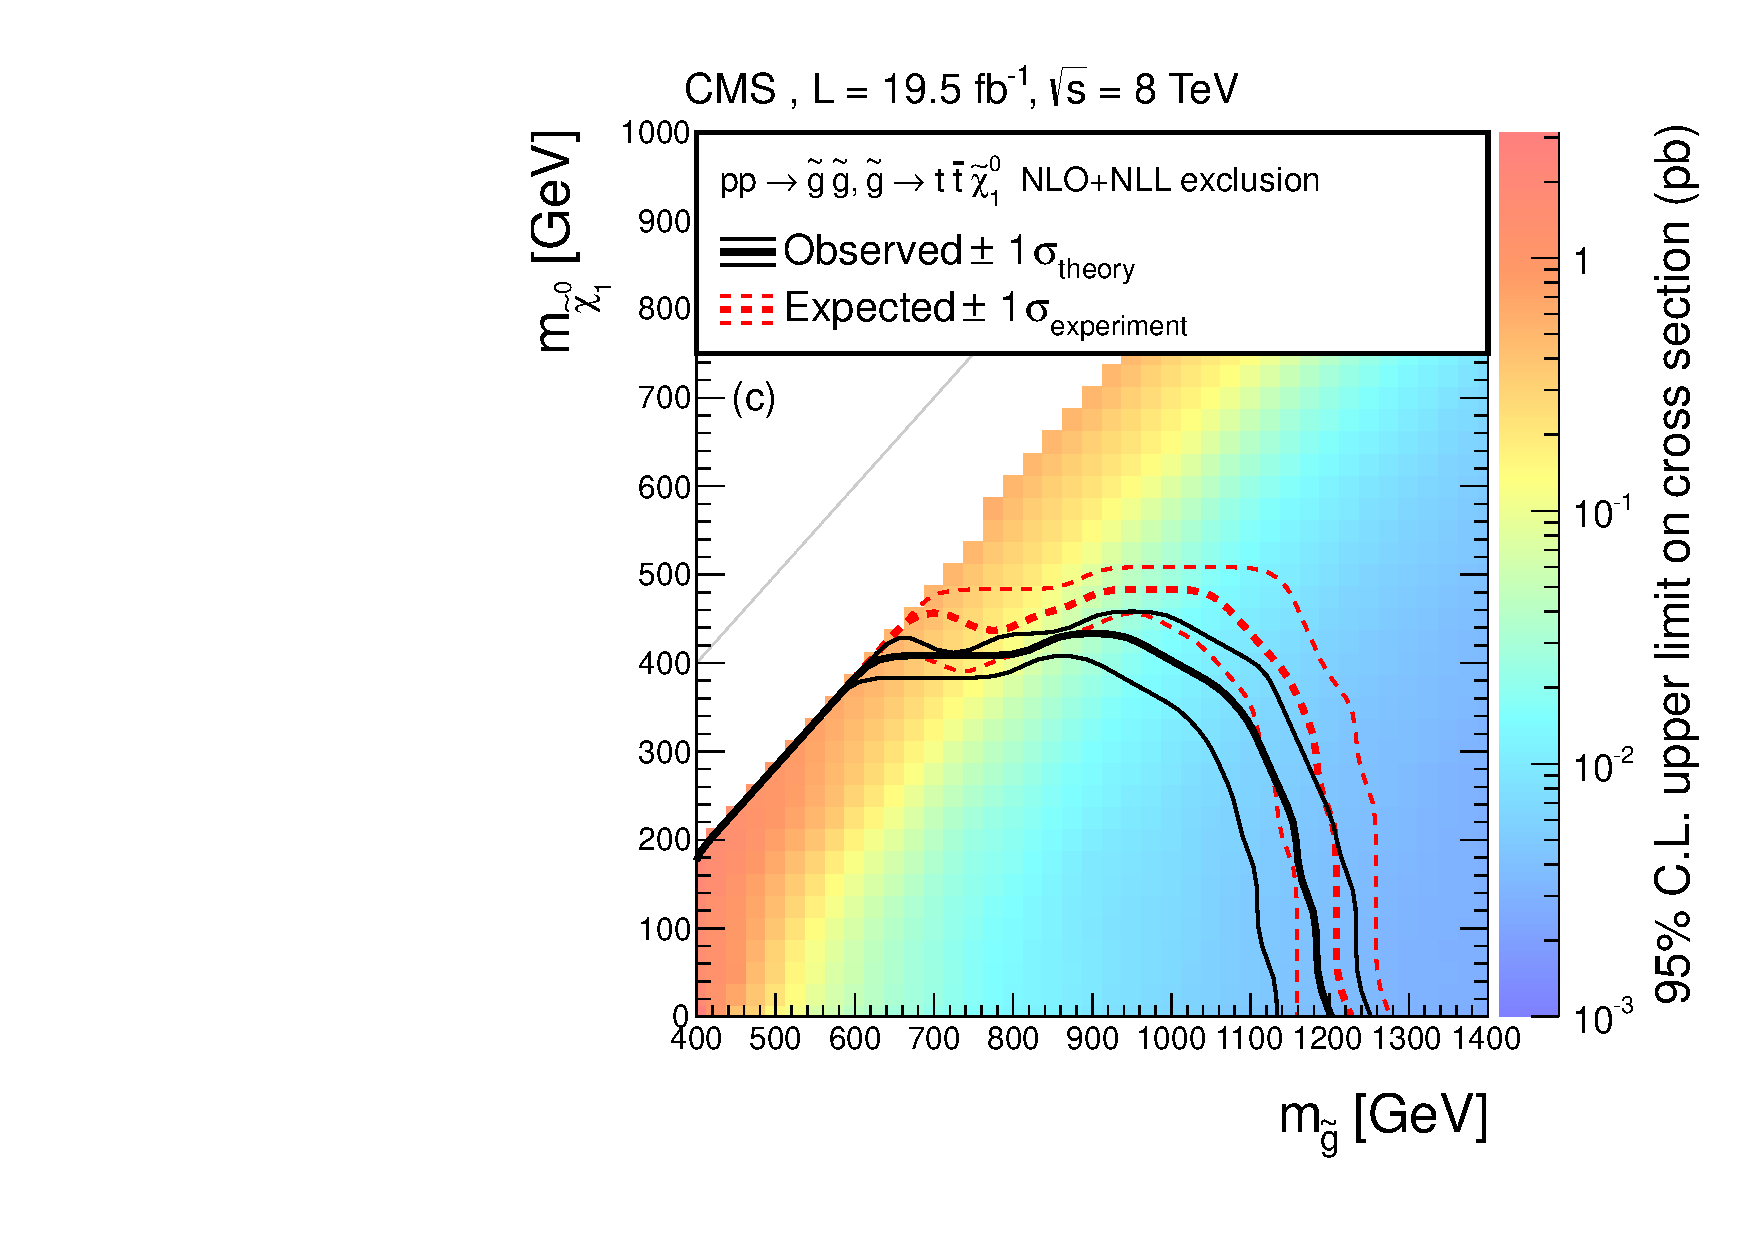
\includegraphics[width=0.42\textwidth]{/home/bibhu/Desktop/PhDThesis/PhDThesis/chapter9/CMS-Limit8TeVT1tttt.pdf}
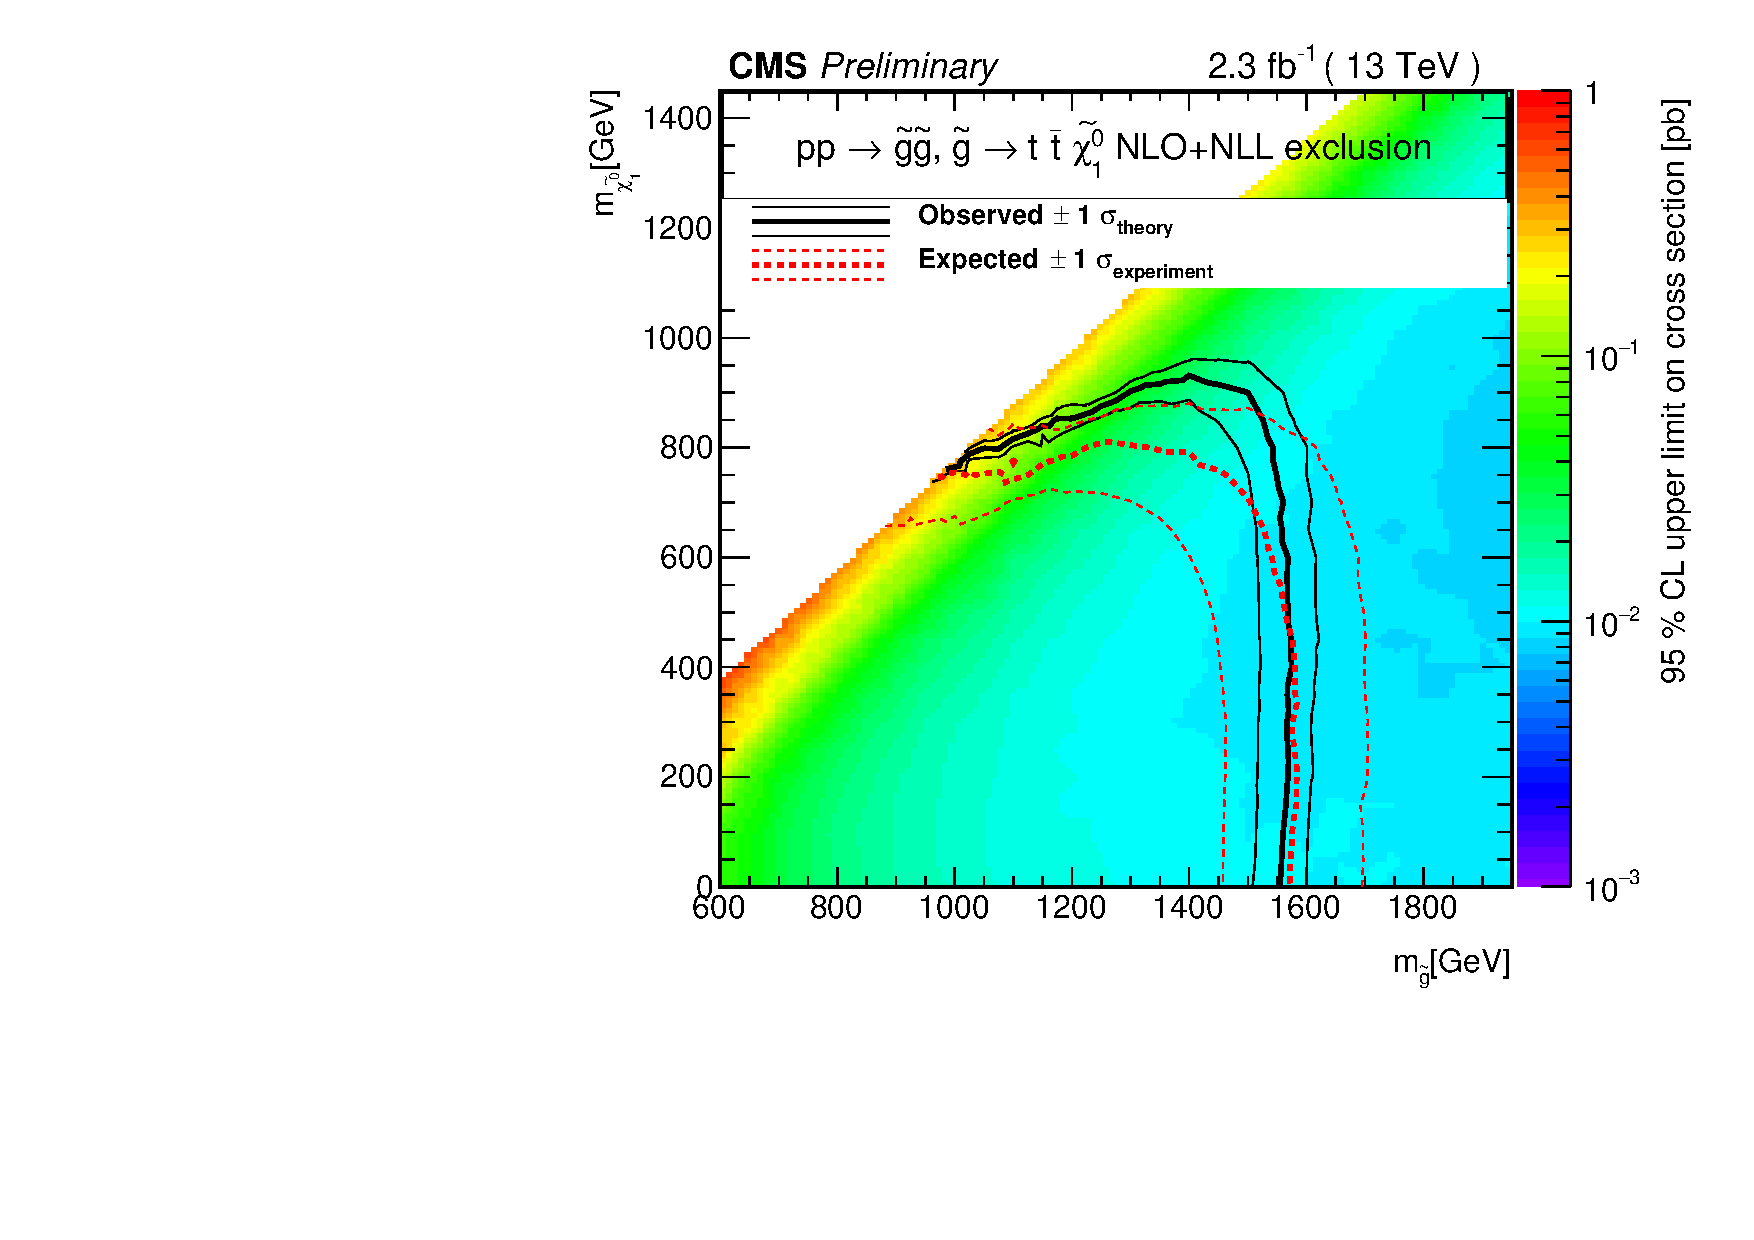
\includegraphics[width=0.47\textwidth]{/home/bibhu/Desktop/PhDThesis/PhDThesis/chapter9/T1tttt_2p3_limit.pdf}
\caption{\label{fig:Limit8vs13SUSY}The 95\% CL upper limits on the gluino pair production cross sections for four top quark final state. The left plot is taken from Ref.~\cite{SUSYhad8TeV}. The right plot is produced by us with 2.3 $\rm fb^{-1}$ of data.}
\end{figure}


Similarly, in the leptoquark analysis we have  extended the previous limits. However, the limits are not improved as much as in SUSY because the increase in SUSY production cross section is much higher going from 8 to 13 TeV as compared to the LQ models. In Fig.~\ref{fig:LQLimit8TeV13TeV}, we present a comparison of the 8TeV limit vis-a-vis the 13 TeV limit. More ever a small excess seen for an LQ mass 650 GeV in the 8TeV analysis ~\cite{CMS-PAS-EXO-12-041} was not confirmed in our analysis indicating the prior signal could be a fluctuation.

\begin{figure}[h]
\centering
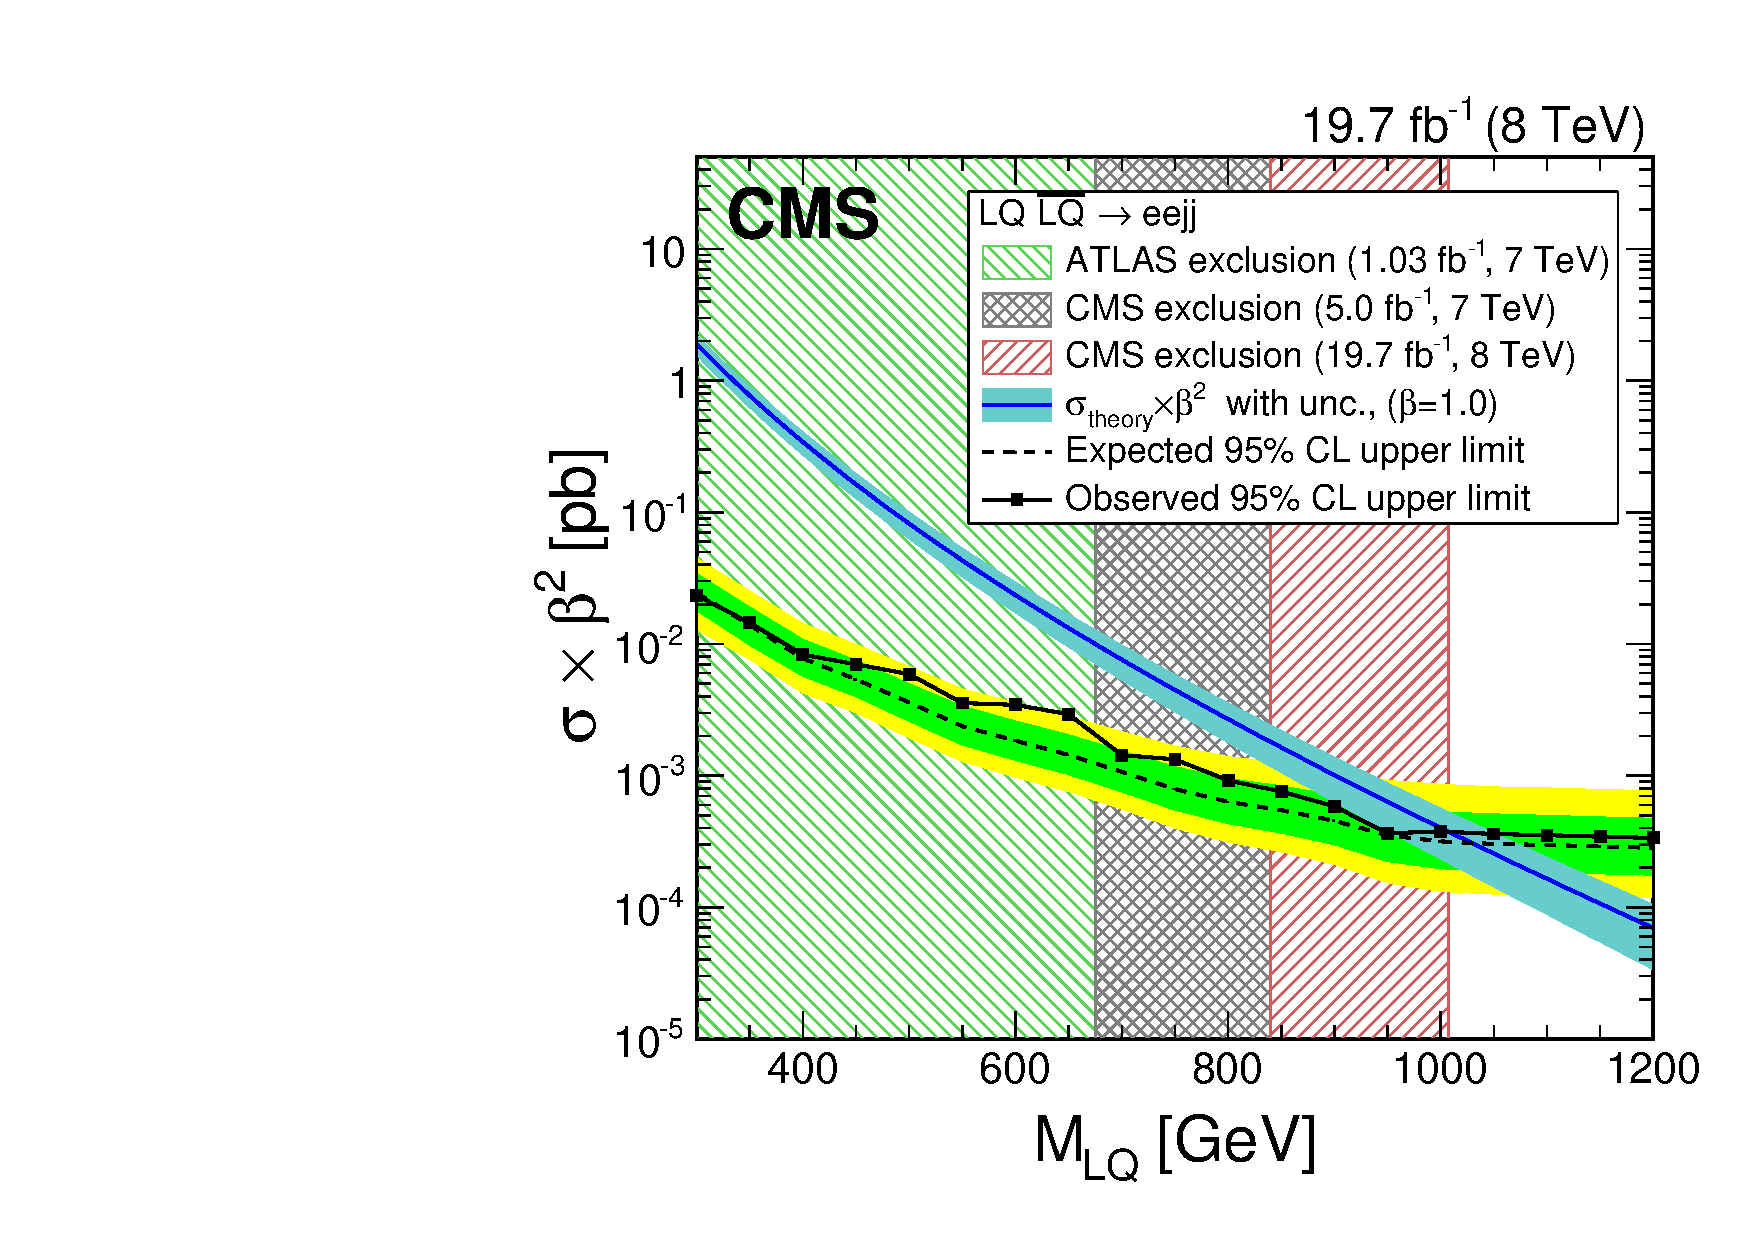
\includegraphics[width=0.42\textwidth]{/home/bibhu/Desktop/PhDThesis/PhDThesis/chapter9/LQ18Tevlimit.pdf}
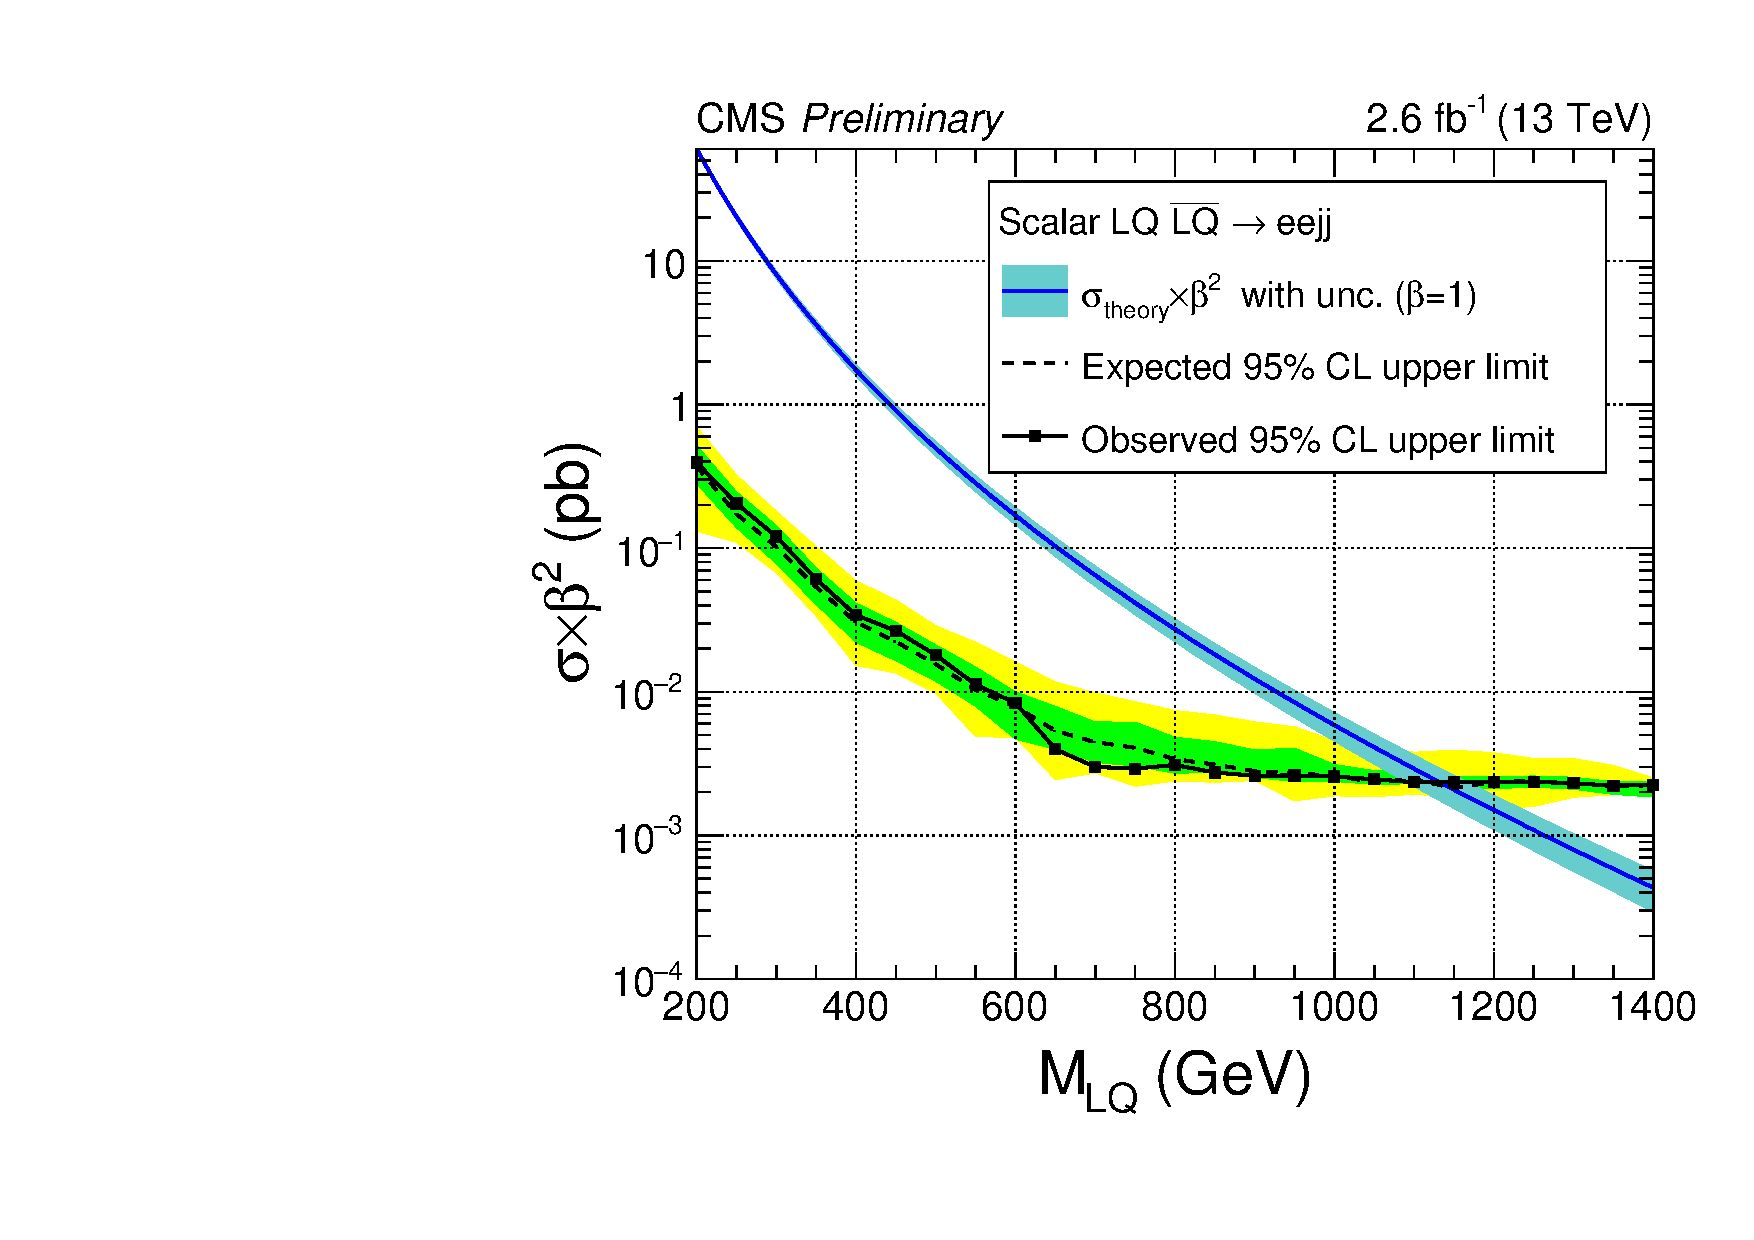
\includegraphics[width=0.42\textwidth]{/home/bibhu/Desktop/PhDThesis/PhDThesis/chapter9/LQLimitPlot.pdf}
\caption{\label{fig:LQLimit8TeV13TeV}The 95\% CL upper limits on the leptoquark production cross section times branching fraction. The left plot is taken from Ref.~\cite{CMS-PAS-EXO-12-041} while the right plot is our result based on 2.6 $\rm fb^{-1}$ of data.}
\end{figure}


At the end, we have presented a study on the various advanced pileup mitigation techniques. It turns out that grooming is very useful when jets are contaminated with pileup. Motivated by our study, many of the current CMS analysises are using grooming techiques for pileup mitigation.

Even though the searches yield null results for new physics, but the results are useful in excluding the parameter space for the SUSY and leptoquarks. But as we understand the SM is incomplete, so there must be new physics at a scale currently not known to us. We believe, with collection of more data with higher energies in the future years could potentialy reveal signatures of new phyisics.  

With this we conclude the presentation of various works that are carried out during our PhD.
































